\documentclass[9pt]{article}

\usepackage{amsmath}
\usepackage{tcolorbox}
% `parskip` removes indentation for all paragraphs: http://tex.stackexchange.com/a/55016
\usepackage{parskip}
% Allows us to color rows / cols of a table.
% See https://texblog.org/2011/04/19/highlight-table-rowscolumns-with-color/
\usepackage{color, colortbl}

\usepackage{graphicx}
\graphicspath{{images/ps3/}}

\usepackage{hyperref}

\leftmargin=0.25in
\oddsidemargin=0.25in
\textwidth=6.0in
\topmargin=-0.25in
\textheight=9.25in

\definecolor{Gray}{gray}{0.9}

\begin{document}

\begin{center}
  \large\textbf{MIT 18.01 Problem Set 3 Unofficial Solutions}
\end{center}

\textbf{NOTE:} This might be the hardest Problem Set in the entire course. Some of the problems here may seem straightforward after you see the solutions - that is not the case when I was solving them and they are anything but straightforward, especially Q3.

I spent a lot amount of time solving the problems in this Problem Set (and I skipped some parts) while I was taking the course, then many weeks after I completed the course, I extracted and refined the relevant stuff from the very messy original work I did on paper, correcting any mistakes found in the process.

If you are in the process of taking this class, don't get too discouraged if you can't solve everything on this Problem Set.

\begin{tcolorbox}
  \textbf{Q2. Hypocycloid.} Show that every tangent line to the curve \( x^{2/3} + y^{2/3} = 1 \) in the first quadrant has the property that portion of the line in the first quadrant has length 1. (Use implicit differentiation; this is the same as problem 45 page 114 of text.)
\end{tcolorbox}

\begin{align*}
  x^{2/3} + y^{2/3} = 1
\end{align*}

Using implicit differentiation with respect to $x$,

\begin{align*}
  \frac{2}{3}x^{-1/3} + \frac{2}{3}y^{-1/3} \cdot \frac{dy}{dx} = 0 \\
  \frac{2}{3}y^{-1/3} \cdot \frac{dy}{dx} = -\frac{2}{3}x^{-1/3} \\
\end{align*}

Assuming $x > 0$, $y > 0$,
\begin{align*}
  \frac{dy}{dx} &= \frac{-\frac{2}{3}x^{-1/3}}{\frac{2}{3}y^{-1/3}} \\
                &= -\frac{x^{-1/3}}{y^{-1/3}} \\
                &= - (\frac{y}{x})^{1/3}
\end{align*}

The tangent line has equation

\begin{align*}
  y - y_0 = -(\frac{y_0}{x_0})^{1/3} (x - x_0)
\end{align*}

for $x_0 > 0, y_0 > 0$ \ . To find the length of the tangent line in the first quadrant, we need to find its x-intercept and y-intercept.

First, the y-intercept. When $x = 0$,

\begin{align*}
  y - y_0 &= -(\frac{y_0}{x_0})^{1/3} (0 - x_0) \\
  y &= y_0 -(\frac{y_0}{x_0})^{1/3} (- x_0) \\
  y &= y_0 + (\frac{y_0}{x_0})^{1/3} x_0 \\
  y &= y_0 + x_0^{2/3} y_0^{1/3}
\end{align*}

Onto the x-intercept. When $y = 0$,

\begin{align*}
  0 - y_0 &= -(\frac{y_0}{x_0})^{1/3}(x - x_0) \\
  y_0 (\frac{x_0}{y_0})^{1/3} &= x - x_0 \\
  x &= x_0 + y_0(\frac{x_0}{y_0})^{1/3} \\
  x &= x_0 + x_0^{1/3} y_0^{2/3}
\end{align*}

So the tangent line cuts the y-axis at $y = y_0 + x_0^{2/3} y_0^{1/3}$ and cuts the x-axis at $x = x_0 + x_0^{1/3} y_0^{2/3}$. We assumed $x_0 > 0, y_0 > 0$ so these 2 coordinates are positive and the length of the tangent line in the first quadrant is simply $\sqrt{x^2 + y^2}$, which is

\begin{align*}
  \sqrt{x^2 + y^2} &= \sqrt{(x_0 + x_0^{1/3} y_0^{2/3})^2 + (y_0 + x_0^{2/3} y_0^{1/3})^2} \\
                   &= \sqrt{x_0^2 + 2x_0^{4/3}y_0^{2/3} + x_0^{2/3} y_0^{4/3} + y_0^2 + 2x_0^{2/3}y_0^{4/3} + x_0^{4/3}y_0^{2/3}} \\
                   &= \sqrt{x_0^2 + y_0^2 + 3x_0^{4/3}y_0^{2/3} + 3x_0^{2/3}y_0^{4/3}} \\
                   &= \sqrt{x_0^{4/3} (x_0^{2/3} + 3y_0^{2/3}) + y_0^{4/3} (y_0^{2/3} + 3x_0^{2/3})} \\
                   &= \sqrt{x_0^{4/3} (x_0^{2/3} + y_0^{2/3} + 2y_0^{2/3}) + y_0^{4/3} (y_0^{2/3} + x_0^{2/3} + 2x_0^{2/3})} \\
                   &= \sqrt{x_0^{4/3} (1 + 2y_0^{2/3}) + y_0^{4/3} (1 + 2x_0^{2/3})} \tag*{(Using $x_0^{2/3} + y_0^{2/3} = 1$)} \\
                   &= \sqrt{x_0^{4/3} + 2x_0^{4/3}y_0^{2/3} + y_0^{4/3} + 2x_0^{2/3}y_0^{4/3}} \\
                   &= \sqrt{2x_0^{2/3}y_0^{2/3} (x_0^{2/3} + y_0^{2/3}) + x_0^{4/3} + y_0^{4/3}} \\
                   &= \sqrt{2x_0^{2/3}y_0^{2/3} + x_0^{4/3} + y_0^{4/3}} \\
                   &= \sqrt{x_0^{2/3} (2y_0^{2/3} + x_0^{2/3}) + y_0^{4/3}} \\
                   &= \sqrt{x_0^{2/3} (x_0^{2/3} + y_0^{2/3} + y_0^{2/3}) + y_0^{4/3}} \\
                   &= \sqrt{x_0^{2/3} (1 + y_0^{2/3}) + y_0^{4/3}} \\
                   &= \sqrt{x_0^{2/3} + x_0^{2/3}y_0^{2/3} + y_0^{4/3}} \\
                   &= \sqrt{y_0^{2/3} (x_0^{2/3} + y_0^{2/3}) + x_0^{2/3}} \\
                   &= \sqrt{y_0^{2/3} + x_0^{2/3}} \\
                   &= \sqrt{1} \\
                   &= 1
\end{align*}

And hence every tangent line to the curve $x_0^{2/3} + y_0^{2/3} = 1$ in the first quadrant has the property that the portion of the line in the first quadrant has length $1$.

\begin{tcolorbox}
  \textbf{Q3. Sensitivity of measurement, revisited.}

  a) Recall that in problem 2, PS1/Part II, $L^2 + 20000^2 = h^2$. Use implicit differentiation to calculate $dL/dh$. Compare the linear approximation $dL/dh$ to the error $\Delta L / \Delta h$ computed in examples on PS1. Explain why $ \Delta L / \Delta h <= dL/dh $ if the derivative is evaluated at the left endpoint of the interval of uncertainty (or, in other words, $\Delta h < 0$). In what range of values of $h$ is it true that $|\Delta L| <= 2|\Delta h|$ ?
\end{tcolorbox}

\begin{tcolorbox}
Use implicit differentiation to find $\frac{dL}{dh}$
\end{tcolorbox}
\begin{align*}
  L^2 + 20000^2 &= h^2 \\
  2L\frac{dL}{dh} &= 2h \\
  \frac{dL}{dh} &= \frac{h}{L}
\end{align*}

\begin{tcolorbox}
  Compare the linear approximation $dL/dh$ to the error $\Delta L / \Delta h$ computed in examples on PS1:
\end{tcolorbox}

This is for $h = 25000$ with altitude $20000$. Then $L = \sqrt{25000^2 - 20000^2} = 15000$ and $\frac{dL}{dh} = \frac{h}{L} = 25000 / 15000 = 5 / 3$.
\begin{center}
  \begin{tabular}{|c|c|c|}
    \hline
    \rowcolor{Gray}
    $\Delta h$ & $\Delta L / \Delta h$ & $\Delta L / \Delta h <= \frac{dL}{dh}$ \\ \hline
    $1$ & $1.666607$ & True \\ \hline
    $10^{-1}$ & $1.666661$ & True \\ \hline
    $10^{-2}$ & $1.666666$ & True \\ \hline
    $-1$ & $1.666726$ & False \\ \hline
    $-10^{-1}$ & $1.666673$ & False \\ \hline
    $-10^{-2}$ & $1.666667$ & False \\ \hline
  \end{tabular}
\end{center}

Now for $h = 20001$ with altitude $20000$. $L = \sqrt{20001^2 - 20000^2} \approx 200.0024999843752$ and $\frac{dL}{dh} = \frac{h}{L} \approx 100.00374996093818$.
\begin{center}
  \begin{tabular}{|c|c|c|}
    \hline
    \rowcolor{Gray}
    $\Delta h$ & $\Delta L / \Delta h$ & $\Delta L / \Delta h <= \frac{dL}{dh}$ \\ \hline
    $1$ & $82.847283$ & True \\ \hline
    $10^{-1}$ & $97.621539$ & True \\ \hline
    $10^{-2}$ & $99.755002$ & True \\ \hline
    $-1$ & $200.002500$ & False \\ \hline
    $-10^{-1}$ & $102.637058$ & False \\ \hline
    $-10^{-2}$ & $100.254998$ & False \\ \hline
  \end{tabular}
\end{center}

\begin{tcolorbox}
  Explain why $\Delta L / \Delta h <= dL / dh$ if the derivative is evaluated at the right endpoint of the interval of uncertainty (or, in other words, $\Delta h > 0$).
\end{tcolorbox}

\textbf{NOTE: There is a typo with this part of the question.} It uses the phrase "left endpoint of the interval of uncertainty" in conjunction with $\Delta h > 0$. It is only after completing the part above where we have more evidence that $\Delta L / \Delta h <= \frac{dL}{dh}$ should be correct and is what the question should be asking for. \\

We have that $L^2 + 20000^2 = h^2$. $L >= 0$, and it's pretty obvious that $h >= 20000$ since $L >= 0$, and that $h > L$. To see how $\frac{h}{L}$ changes according to a change in $h$, we take limits on both ends of $h$.

\begin{equation*}
  \lim_{h\to20000^+} \frac{h}{L} = \lim_{h\to20000^+} \frac{h}{\sqrt{h^2 - 20000^2}}
                                 = \lim_{h\to20000^+} \sqrt{\frac{h^2}{h^2 - 20000^2}}
                                 = \lim_{h\to20000^+} \sqrt{\frac{h^2 / h^2}{h^2 / h^2 - 20000^2 / h^2}} \\
\end{equation*}
\begin{equation*}
  = \lim_{h\to20000^+} \sqrt{\frac{1}{1 - (\frac{20000}{h})^2}} = \infty
\end{equation*}
\begin{equation*}
  \lim_{h\to\infty} \frac{h}{L} = \lim_{h\to\infty} \sqrt{\frac{1}{1 - (\frac{20000}{h})^2}} = \sqrt{\frac{1}{1 - 0}} = 1
\end{equation*}

So we can conclude that $\frac{h}{L} >= 1$. Now, going back to $L^2 + 20000^2 = h^2$, suppose we add $\Delta h > 0$ to $h$. Then the resulting $L$ will be $L + \Delta L$ for some $\Delta L > 0$.

\begin{align*}
  (h + \Delta h)^2 &= (L + \Delta L)^2 + 20000^2 \\
  h + \Delta h &= \sqrt{(L + \Delta L)^2 + 20000^2} \\
  \Delta h &= \sqrt{(L + \Delta L)^2 + 20000^2} - h \\
           &= \sqrt{L^2 + 2L\Delta L + (\Delta L)^2 + 20000^2} - h \\
           &= \sqrt{(L^2 + 20000^2) + 2L\Delta L + (\Delta L)^2} - h \\
           &= \sqrt{h^2 + 2L\Delta L + (\Delta L)^2} - h \\
           &<= \sqrt{h^2 + 2h\Delta L + (\Delta L)^2} - h \tag*{(Since $h >= L$ and $\Delta L > 0$)} \\
           &= \sqrt{(h + \Delta L)^2} - h \\
           &= h + \Delta L - h \\
           &= \Delta L
\end{align*}

And $\Delta L >= \Delta h$. Since both $\Delta h > 0$ and $\Delta L > 0$, we have that $\frac{\Delta L}{\Delta h} >= 1$.  Earlier we proved that $\frac{h}{L} >= 1$. Unfortunately, these 2 facts combined \textbf{cannot} help us prove that $\frac{\Delta L}{\Delta h} <= \frac{dL}{dh} = \frac{h}{L}$ for $\Delta h > 0$. In fact, you can try adding $\Delta h < 0$ (which means $\Delta L < 0$) and reach the same conclusion that $\frac{\Delta L}{\Delta h} >= 1$. That is also what we observe when computing the values for $\frac{\Delta L}{\Delta h}$ in the tables above. \\

We shall instead offer a more hand-wavy explanation for the phenomenon (which may be wrong). I have tried extremely hard to reason about this problem for a long time and this is the only sufficiently reasonable explanation I can come up with.\\

Earlier, we proved that $\lim_{h \rightarrow 20000^+} \frac{h}{L} = \infty$ and $\lim_{h \rightarrow \infty} \frac{h}{L} = 1$. Since $\frac{dL}{dh} = \frac{h}{L}$, the rate of change of $L$ with respect to $h$ is decreasing (but positive) as $h$ increases. As such, for $\Delta h > 0$, $\frac{\Delta L}{\Delta h}$, which is the actual change in $L$ over the actual change in $h$, decreases as $\Delta h$ increases. In fact, due to the decreasing $\frac{dL}{dh}$, $\Delta L <= \frac{dL}{dh} * \Delta h$ for $\Delta h > 0$, which gives us $\frac{\Delta L}{\Delta h} <= \frac{dL}{dh} = \frac{h}{L}$.

\begin{tcolorbox}
  In what range of values of $h$ is it true that $|\Delta L| <= 2|\Delta h|$ ?
\end{tcolorbox}

$|\Delta L| <= 2|\Delta h|$ implies that $\frac{|\Delta L|}{|\Delta h|} <= 2$, which implies that $|\frac{\Delta L}{\Delta h}| <= 2$. We know that $\Delta L$ and $\Delta h$ have the same sign, so this simplifies to $\frac{\Delta L}{\Delta h} <= 2$.

For $\Delta h > 0$, we have $\frac{\Delta L}{\Delta h} <= \frac{dL}{dh} = \frac{h}{L}$. Therefore, we need to find $h$ such that $\frac{h}{L} <= 2$.

\begin{align*}
  \frac{h}{L} &<= 2 \\
  h &<= 2L \\
    &= 2\sqrt{h^2 - 20000^2}
\end{align*}

Squaring both sides,

\begin{align*}
  h^2 &<= 4(h^2 - 20000^2) \\
  3h^2 &>= 4 * 20000^2 \\
  h^2 &>= \frac{4 * 20000^2}{3} \\
  h &>= \sqrt{\frac{4 * 20000^2}{3}} \approx 23094.010760368154
\end{align*}

But that is just for $\Delta h > 0$. How about for $\Delta h < 0$? We also require that $\frac{\Delta L}{\Delta h} <= 2$. Since $\Delta h$ and $\Delta L$ have the same sign, we want to find $\Delta h < 0$ that will result in the highest magnitude $\Delta L$.

Earlier we proved that $\frac{dL}{dh} = \frac{h}{L}$ and $\lim_{h \rightarrow 20000^+} \frac{h}{L} = \infty$ and $\lim_{h \rightarrow \infty} \frac{h}{L} = 1$. Hence $\frac{dL}{dh}$ is decreasing (but positive) as $h$ increases. Hence for $\Delta h < 0$, it makes sense that the maximum $|\Delta L|$ arises from a change in $h$ that brings it all the way back to its minimum allowed value of $20000$. In other words, $\Delta h = -(h - 20000)$. The corresponding value of $\Delta L$ is then $-L$, because if $h$ goes back to $20000$, the constraint $L^2 + 20000^2 = h^2$ causes $L$ to go to $0$. Then $\frac{\Delta L}{\Delta h} = \frac{-L}{-(h - 20000)} = \frac{L}{h - 20000}$ and we require this to be less than or equal to $2$.

\begin{align*}
  \frac{L}{h - 20000} &<= 2 \\
  L &<= 2(h - 20000) \\
  \sqrt{h^2 - 20000^2} &<= 2h - 40000 \\
  h^2 - 20000^2 &<= (2h - 40000)^2 \\
  h^2 &<= 4h^2 - 160000h + 40000^2 + 20000^2 \\
  3h^2 - 160000h + 2*10^9 &>= 0
\end{align*}

Let $y = 3h^2 - 160000h + 2*10^9$. We solve for $y = 0$, getting $h = \frac{-(-160000) + \sqrt{(-160000)^2 - 4 \cdot 3 \cdot 2 * 10^9}}{2 * 3}$, getting $h = 33333.333333333336$ and $h = 20000$. $\frac{dy}{dh} = 6h - 160000$. At the critical points, $6h - 160000 = 0$ so $h = \frac{160000}{6} = 26666 \frac{2}{3}$. $\frac{d^2 y}{dh^2} = 6 > 0$ so $h = 26666 \frac{2}{3}$ is a minimum point. At $h = 26666 \frac{2}{3}, y = -133333332 < 0$.

This is a pretty "standard" quadratic function, so $y >= 0$ for $h <= 20000$ and $y <= 0$ for $20000 <= h <= 33333 \frac{1}{3}$ and $y >= 0$ for $h >= 33333 \frac{1}{3}$. By the constraints of the problem, $h$ must be at least $20000$, so we need to take $h >= 33333 \frac{1}{3}$. Then $\frac{\Delta L}{\Delta h} <= \frac{L}{h - 20000} <= 2$ for $\Delta h < 0$. Since $33333 \frac{1}{3} > 23094.010760368154$, for $h >= 33333 \frac{1}{3}$, we will also have $\frac{\Delta L}{\Delta h} <= 2$ for $h > 0$.

Hence for $|\Delta L| <= 2 |\Delta h|$ or equivalently $\frac{\Delta L}{\Delta h} <= 2$, we need $h >= 33333 \frac{1}{3}$.
 
\begin{tcolorbox}
  \textbf{Q3. Sensitivity of measurement, revisited.}

  b) Suppose that the Planet Quirk is a not only flat, but one-dimensional (a straight line). There are several satellites at height $20,000$ kilometres and you get readings saying that satellite 1 is directly above the point $x_1 \pm 10^{-10}$ and is at a distance $h_1 = 21,000 \pm 10^{-2}$ from you, satellite 2 is directly above $x_2 \pm 10^{-10}$ and at a distance $h_2 = 52,000 \pm 10^{-2}$. Where are you and to what accuracy? Hint: Consider separately the cases $x1 < x2$ and $x2 > x1$.
\end{tcolorbox}

\textbf{NOTE:} I am only doing 1 part of this question and I'm not sure whether my solution is correct. This question also covers propagation of error, which is not covered in the lectures.

Suppose we are at point $q$ of Planet Quirk. We'll follow the hint given in this question.

\textbf{Case 1:} $x_1 < x_2$

\textbf{Case 1a:} $q < x_1 < x_2$

We can safely ignore $q = x_1$, because if $q = x_1$, $h_1 = 20,000$ but that is not the case.

Let's ignore the uncertainties in measurement. Then we have the following equations:

\begin{align}
  (x_1 - q)^2 &= h_1^2 - 20000^2 \\
  (x_2 - q)^2 &= h_2^2 - 20000^2
\end{align}

From the above 2 equations we see that

\begin{align}
  q = x_1 - \sqrt{h_1^2 - 20000^2} \\
  q = x_2 - \sqrt{h_2^2 - 20000^2}
\end{align}

In general, we see that given an $x$ and $h$, we have $q = x - \sqrt{h^2 - 20000^2}$

If these YouTube videos are correct and I've interpreted their content correctly:

\url{https://www.youtube.com/watch?v=N0OYaG6a51w} \\
\url{https://www.youtube.com/watch?v=V0ZRvvHfF0E}

we can treat $x$ and $h$ as variables, get their partial derivatives, and compute the uncertainty in $q$ as follows:

\begin{align*}
  \Delta q = \sqrt{(\frac{\partial q}{\partial x} \cdot \Delta x)^2 + (\frac{\partial q}{\partial h} \cdot \Delta h)^2}
\end{align*}

Now, $\frac{\partial q}{\partial x} = 1$ and $\frac{\partial q}{\partial h} = -\frac{1}{2} \cdot 2h \cdot (h^2 - 20000^2)^{-1/2} = -\frac{h}{\sqrt{h^2 - 20000^2}}$.

Based on $x_1$, $\Delta x_1 = \pm 10^-10$, $h_1 = 21000$, $\Delta h_1 = 10^{-2}$,

\begin{align*}
  \Delta q &= \sqrt{(1 \cdot \pm 10^{-10})^2 + (-\frac{21000}{21000^2 - 20000^2} \cdot \pm 10^{-2})^2} \\
           &= \sqrt{10^{-20} + \frac{21000^2}{21000^2 - 20000^2} \cdot 10^{-4}} \\
           &\approx 0.03162277660168379
\end{align*}

Then

\begin{align*}
  q &= x_1 - \sqrt{h_1^2 - 20000^2} \pm \Delta q \\
    &= x_1 - \sqrt{21000^2 - 20000^2} \pm \Delta q \\
    &\approx x_1 - 6403.1242374328485 \pm 0.03162277660168379
\end{align*}

Based on $x_2$, $\Delta x_2 = \pm 10^-10$, $h_2 = 52000$, $\Delta h_2 = 10^{-2}$,

\begin{align*}
  \Delta q &= \sqrt{(1 \cdot \pm 10^{-10})^2 + (-\frac{52000}{52000^2 - 20000^2} \cdot \pm 10^{-2})^2} \\
           &= \sqrt{10^{-20} + \frac{52000^2}{52000^2 - 20000^2} \cdot 10^{-4}} \\
           &\approx 0.01
\end{align*}

Then

\begin{align*}
  q &= x_2 - \sqrt{h_2^2 - 20000^2} \pm \Delta q \\
    &= x_2 - \sqrt{52000^2 - 20000^2} \pm \Delta q \\
    &\approx x_2 - 48000 \pm 0.01
\end{align*}

Now, I believe that these 2 measurements of $q$ along with uncertainty $\Delta q$ should partially overlap and the interval of $q$ should be the intersection of these 2 intervals. I also believe that it is a contradiction if the intervals are non overlapping. However, I am not able to prove either of that.

This is also the only case in this part of the question I will tackle. I have spent waaaaay too much time on this Problem Set and this is the final part of the Problem Set I worked on in my writeup. Apologies to readers for the incompleteness.

\begin{tcolorbox}
  \textbf{Q3. Sensitivity of measurement, revisited.}

  c) Express $dL/dh$ in terms of the angle between the line of sight to the satellite and the horizontal from the person on the ground. (When expressed using the line-of-sight angle, the formula also works for a curved planet like Earth.)
\end{tcolorbox}

\textbf{Note to reader:} I'm not sure whether my solution to this part is correct.

\begin{align*}
  cos \theta &= \frac{L}{h}
\end{align*}

Differentiating implicitly wrt $h$,

\begin{align*}
  -sin\theta \cdot \frac{d\theta}{dh} &= \frac{dL}{dh} \cdot \frac{1}{h} + L \cdot (-\frac{1}{h^2}) \\
  \frac{dL}{dh} &= (-sin\theta \cdot \frac{d\theta}{dh} + \frac{L}{h^2}) * h \\
                &= \frac{L}{h} - h \cdot sin\theta \cdot \frac{d\theta}{dh}
\end{align*}



\begin{tcolorbox}
  \textbf{Q4. More sensitivity of measurement.}

  Consder a parabolic mirror with equation $y = -1/4 + x^2$ and focus at the origin. (See Problem Set 1.) A ray of light traveling down vertically along the line $x = a$ hits the mirror at the point $(a, b)$ where $b = -1/4 + a^2$ and goes to the origin along a ray at angle $\theta$ measured from the positive x-axis.

  a) Find the formula for $tan\theta$ in terms of $a$ and $b$, and calculate $d\theta / da$ using implicit differentiation. (Express your answer in terms of $a$ and $\theta$.)
\end{tcolorbox}

Assuming $a \neq 0$, $tan \theta = \frac{b}{a} = \frac{-1/4 + a^2}{a} = a - \frac{1}{4a}$

Differentiating implicitly with respect to $a$,

\begin{align*}
  (sec^2 \theta) \cdot \frac{d \theta}{da} &= 1 + \frac{1}{4a^2} \\
  \frac{d \theta}{da} &= cos^2 \theta (1 + \frac{1}{4a^2}) \\
                      &= cos^2 \theta + \frac{cos^2 \theta}{4a^2}
\end{align*}

\begin{tcolorbox}
  \textbf{Q4. More sensitivity of measurement.}

  b) If the telescope records a star at $\theta = -\pi / 6$ and the measurement is accurate to $10^{-3}$ radians, use part (a) to give an estimate as to the location of the star in the variable $a$.
\end{tcolorbox}

\textbf{NOTE:} This makes use of propagation of error, which isn't really covered in the lectures.

Since we are given $\theta$ and its accuracy, we actually want $\frac{da}{d \theta}$.

\begin{align*}
  tan \theta &= a - \frac{1}{4a} \\
  sec^2 \theta &= \frac{da}{d \theta} + \frac{1}{4a^2} \cdot \frac{da}{d \theta} \\
  sec^2 \theta &= \frac{da}{d \theta} (1 + \frac{1}{4a^2}) \\
  da &= \frac{sec^2 \theta}{(1 + \frac{1}{4a^2})} \cdot d \theta \\
     &= \frac{sec^2 \theta}{\frac{4a^2 + 1}{4a^2}} \cdot d \theta \\
     &= \frac{4a^2 sec^2 \theta}{4a^2 + 1} \cdot d \theta \\
     &= \frac{4a^2}{cos^2 \theta (4a^2 + 1)} \cdot d \theta
\end{align*}

which turns out to be exactly the same thing as if we started from what we have in part (a):

\begin{align*}
  \frac{d \theta}{da} &= cos^2 \theta + \frac{cos^2 \theta}{4a^2} \\
  da &= \frac{1}{cos^2 \theta + \frac{cos^2 \theta}{4a^2}} \cdot d \theta \\
     &= \frac{1}{\frac{4a^2 cos^2 \theta + cos^2 \theta}{4a^2}} \cdot d \theta \\
     &= \frac{4a^2}{4a^2 cos^2 \theta + cos^2 \theta} \cdot d \theta \\
     &= \frac{4a^2}{cos^2 \theta (4a^2 + 1)} \cdot d \theta
\end{align*}

At $\theta = -\frac{\pi}{6}$, $tan \theta = tan (-\frac{\pi}{6}) = -\frac{1}{\sqrt{3}}$. But $tan \theta = a - \frac{1}{4a}$. Hence

\begin{align*}
  -\frac{1}{\sqrt{3}} &= a - \frac{1}{4a} \\
  (-\frac{1}{\sqrt{3}})^2 &= (\frac{a \cdot 4a - 1}{4a})^2 \\
  \frac{1}{3} &= (\frac{4a^2 - 1}{4a})^2 \\
  \frac{1}{3} &= \frac{16a^4 - 8a^2 + 1}{16a^2} \\
  16a^2 &= 3(16a^4 - 8a^2 + 1) \\
  48a^4 - 24a^2 + 3 - 16a^2 &= 0 \\
  48a^4 - 40a^2 + 3 &= 0 \\
  a^2 &= \frac{-(-40) \pm \sqrt{(-40)^2 - 4 \cdot 48 \cdot 3}}{2 \cdot 48} \\
      &= \frac{40 \pm \sqrt{1024}}{96} \\
      &= \frac{40 \pm 32}{96}
\end{align*}

So $a^2 = \frac{40 + 32}{96} = \frac{72}{96} = \frac{3}{4}$ or $a^2 = \frac{40 - 32}{96} = \frac{8}{96} = \frac{1}{12}$.

Then $a = \pm \frac{\sqrt{3}}{2}$ or $a = \pm \frac{1}{\sqrt{12}} = \pm \frac{1}{\sqrt{3 * 4}} = \pm \frac{1}{2 \sqrt{3}} = \pm \frac{\sqrt{3}}{6}$.

When $a = \frac{\sqrt{3}}{2}$, $da = \frac{4a^2}{cos^2 \theta (4a^2 + 1)} \cdot d \theta = \frac{4 (\frac{\sqrt{3}}{2})^2}{cos^2 (-\frac{\pi}{6}) (4 \cdot (\frac{\sqrt{3}}{2})^2 + 1)} \cdot d \theta = \frac{4 \cdot \frac{3}{4}}{(\frac{\sqrt{3}}{2})^2 (4 \cdot \frac{3}{4} + 1)} \cdot d \theta = \frac{3}{\frac{3}{4} (3 + 1)} \cdot d \theta = \frac{3}{3} \cdot d \theta = d \theta$. This is also the same for $a = -\frac{\sqrt{3}}{2}$. Hence for $a = \pm \frac{\sqrt{3}}{2}, da = d \theta = 10^{-3}$.

When $a = \frac{\sqrt{3}}{6}, da = \frac{4a^2}{cos^2 \theta (4a^2 + 1)} \cdot d \theta = \frac{4 (\frac{\sqrt{3}}{6})^2}{cos^2 (-\frac{\pi}{6}) (4 \cdot (\frac{\sqrt{3}}{6})^2 + 1)} \cdot d \theta = \frac{4 \cdot \frac{3}{36}}{(\frac{\sqrt{3}}{2})^2 (4 \cdot \frac{3}{36} + 1)} \cdot d \theta = \frac{\frac{3}{9}}{\frac{3}{4}(\frac{3}{9} + 1)} \cdot d \theta = \frac{\frac{3}{9}}{\frac{3}{4} \cdot \frac{12}{9}} \cdot d \theta = \frac{1}{3} d \theta$. This is also the same for $a = -\frac{\sqrt{3}}{6}$. Hence for $a = \pm \frac{\sqrt{3}}{6}, da = \frac{1}{3} d \theta = \frac{1}{3} \cdot 10^{-3}$.

\begin{tcolorbox}
  \textbf{Q4. More sensitivity of measurement.}

  c) (optional; no credit) Solve for $a$ as a function of $\theta$ alone and doublecheck your answers to parts (a) and (b).
\end{tcolorbox}

\begin{align*}
  tan \theta &= a - \frac{1}{4a} \\
  tan \theta &= \frac{4a^2 - 1}{4a} \\
  4a \cdot tan \theta &= 4a^2 - 1 \\
  4a^2 - 4 (tan \theta) \cdot a - 1 &= 0 \\
  a &= \frac{-(-4 \cdot tan \theta) \pm \sqrt{(-4 \cdot tan \theta)^2 - 4 \cdot 4 \cdot (-1)}}{2 \cdot 4} \\
    &= \frac{4 \cdot tan \theta \pm \sqrt{16 \cdot tan^2 \theta + 16}}{8} \\
    &= \frac{4 \cdot tan \theta \pm \sqrt{16 sec^2 \theta}}{8} \\
    &= \frac{4 \cdot tan \theta \pm 4 \cdot sec \theta}{8} \\
    &= \frac{tan \theta \pm sec \theta}{2}
\end{align*}

\textbf{Case 1:} $a = \frac{tan \theta + sec \theta}{2} = \frac{tan (-\frac{\pi}{6}) + sec (-\frac{\pi}{6})}{2} = \frac{-\frac{1}{\sqrt{3}} + \frac{2}{\sqrt{3}}}{2} = \frac{\frac{1}{\sqrt{3}}}{2} = \frac{1}{2 \sqrt{3}} = \frac{\sqrt{3}}{6}$

\begin{align*}
  \frac{da}{d \theta} &= \frac{sec^2 \theta + sec \theta tan \theta}{2} \\
  da &= \frac{1}{2} (sec^2 \theta + sec \theta tan \theta) \cdot d \theta \\
     &= \frac{1}{2} (sec^2 (-\frac{\pi}{6}) + sec(-\frac{\pi}{6}) tan(-\frac{\pi}{6})) \cdot d \theta \\
     &= \frac{1}{2} ((\frac{2}{\sqrt{3}})^2 + \frac{2}{\sqrt{3}}(-\frac{1}{\sqrt{3}})) \cdot d \theta \\
     &= \frac{1}{2} (\frac{4}{3} - \frac{2}{3}) \cdot d \theta \\
     &= \frac{1}{2} \cdot \frac{2}{3} \cdot d \theta \\
     &= \frac{1}{3} d \theta
\end{align*}

which agrees with what we've got in part (b).

\textbf{Case 2:} $a = \frac{tan \theta - sec \theta}{2} = \frac{tan (-\frac{\pi}{6}) - sec (-\frac{\pi}{6})}{2} = \frac{-\frac{1}{\sqrt{3}} - \frac{2}{\sqrt{3}}}{2} = \frac{-\frac{3}{\sqrt{3}}}{2} = -\frac{3}{2 \sqrt{3}} = -\frac{3 \sqrt{3}}{6} = -\frac{\sqrt{3}}{2}$

\begin{align*}
  \frac{da}{d \theta} &= \frac{sec^2 \theta - sec \theta tan \theta}{2} \\
  da &= \frac{1}{2} (sec^2 \theta - sec \theta tan \theta) \cdot d \theta \\
     &= \frac{1}{2} (sec^2 (-\frac{\pi}{6}) - sec(-\frac{\pi}{6}) tan(-\frac{\pi}{6})) \cdot d \theta \\
     &= \frac{1}{2} ((\frac{2}{\sqrt{3}})^2 - \frac{2}{\sqrt{3}}(-\frac{1}{\sqrt{3}})) \cdot d \theta \\
     &= \frac{1}{2} (\frac{4}{3} + \frac{2}{3}) \cdot d \theta \\
     &= \frac{1}{2} \cdot 2 \cdot d \theta \\
     &= d \theta
\end{align*}

which agrees with what we've got in part (b).

\begin{tcolorbox}
  \textbf{Q5. Newton's method} \\
  a) Compute the cube root of 9 to 6 significant figures using Newton's method. Give the general formula, and list numerical values, starting with $x_0 = 2$. At what iteration $k$ does the method surpass the accuracy of your calculator or computer? (Display your answers to the accuracy of your calculator or computer.)
\end{tcolorbox}

Let $x = \sqrt[3]{9}$. This is our quantity of interest. But we need to convert this to something we can solve using Newton's method. Cubing both sides, we have $x^3 = 9$ and hence $x^3 - 9 = 0$.

Recall that the formula for Newton's method is given by $x_{n+1} = x_n - \frac{y_n}{f'(x_n)} = x_n - \frac{f(x_n)}{f'(x_n)}$, where $x_n$ is the $n$th guess. In this case, $f(x) = x^3 - 9$ and $f'(x) = \frac{d}{dx} x^3 - 9 = 3x^2$. Since $2^3 = 8$ is close to 9 and is a cube that we know, let's use use $x_0 = 2$ as our initial guess.

\begin{center}
  \begin{tabular}{|c|c|c|c|}
    \hline
    \rowcolor{Gray}
    $n$ & $x_n$ & $|f(x_n) - 9|$ & $|x_n - \sqrt[3]9|$ \\ \hline
    0 & 2 & $|2^3 - 9| = 1$ & $|2 - \sqrt[3]9| \approx 0.080084$ \\ \hline
    1 & $2 - \frac{2^3 - 9}{3\cdot2^2} = 2 + \frac{1}{12} = \frac{25}{12}$ & $|(\frac{25}{12})^3 - 9| \approx 0.042245$ & $|\frac{25}{12} - \sqrt[3]9| \approx 0.003250$  \\ \hline
    2 & $\frac{25}{12} - \frac{(25/12)^3 - 9}{3\cdot (25/12)^2} \approx 2.080088888888889$ & $6.575597 * 10^{-5}$ & $\approx 5.065837*10^{-06}$ \\ \hline
    3 & $2.0800838230642413$ & $1.601403* 10^{-10}$ & $\approx 1.233724*10^{-11}$ \\ \hline
    4 & $2.080083823051904$ & $0.0$ & $0.0$ \\ \hline
  \end{tabular}
\end{center}

Calculations done using Python 2.7 . I've truncated the numbers for the final 2 columns to 6 decimal places. So we see that by iteration 5 (at $n = 4$), both ${x_n}^3 - 9$ and $x_n - \sqrt[3]9$ exceed Python 2.7's accuracy. Which is pretty fast. In fact, this happens by iteration 3 for a handheld calculator I'm using.

\begin{tcolorbox}
  \textbf{Q5. Newton's method} \\
  b) For each step $x_k, \ k = 0, 1, ... ,$ say whether the value is i) larger or smaller than $9^{1/3}$; ii) larger or smaller than the perceding value $x_{k-1}$. Illustrate on the graph $x^3 - 9$ why this is so.
\end{tcolorbox}

\begin{center}
  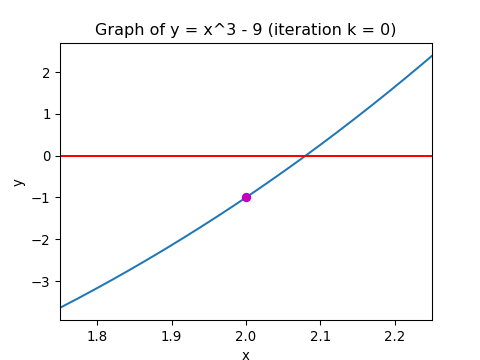
\includegraphics[scale=0.8]{k_eq_0.png}
\end{center}

The graph in blue is $x^3 - 9$. The point in magenta is $x_0 = 2$ plugged into $y = x^3 - 9$. The point where the red line $y = 0$ cuts the curve $y = x^3 - 9$ represents the number $\sqrt[3]9$. We see that $x_0 < \sqrt[3]9$. It should be obvious that the gradient of $y = x^3 - 9$ at $x_0 = 2$ is positive and the $y_0 = 2^3 - 9 = -1$ is negative. Hence $x_1 = x_0 - \frac{x_0}{f'(x_0)}$ is a positive value and $x_1 > x_0$.

\begin{center}
  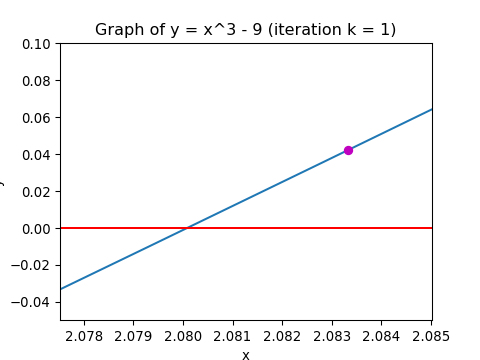
\includegraphics[scale=0.8]{k_eq_1.png}
\end{center}

For $k = 1$, we see that $f(x_1) = x_1^3 - 9 > 0$ and $f'(x_1) > 0$ and hence $\frac{f(x_1)}{f'(x_1)}$ is a positive quantity, so $x_2 = x_1 - \frac{f(x_1)}{f'(x_1)} < x_1$.

It is not very meaningful to carry on for $k > 1$ because Newton's method converges very quickly in this case and I believe you get the idea from these 2 iterations.

\begin{tcolorbox}
  \textbf{Q5. Newton's method} \\
  c) Find a quadratic approximation to $9^{1/3}$, and estimate the difference between the quadratic approximation and the exact answer. (Hint: To get a reasonable quadratic approximation, use $9 = 8(1 + 1/8)$.)
\end{tcolorbox}

\begin{align*}
  \sqrt[3]9 = (8 + 1)^{1/3} = (8(1 + \frac{1}{8}))^{1/3} = 2\cdot(1 + \frac{1}{8})^{1/3}
\end{align*}

Since $\frac{1}{8}$ is kind of small, we will use the quadratic approximation to $2(1 + x)^{1/3}$ where $x = \frac{1}{8}$ to get an approximation to $\sqrt[3]9$.

Let's first derive the quadratic approximation to $(1+x)^r$ for $x$ near 0.

\begin{align*}
  (1 + x)^r &\approx (1 + 0)^r + r(1 + 0)^{r-1}x + \frac{r(r-1)(1+0)^{r-2}}{2!}x^2 \\
            &= 1 + rx + \frac{r(r-1)}{2}x^2
\end{align*}

Substitute $x = \frac{1}{8}, r = \frac{1}{3}$ into $(1 + x)^r$, we get:

\begin{align*}
  (1 + \frac{1}{8})^{1/3} &= 1 + \frac{1}{3} \cdot \frac{1}{8} + \frac{\frac{1}{3}(-\frac{2}{3})}{2}(\frac{1}{8})^2 \\
                          &= 1 + \frac{1}{24} - \frac{1}{9} \cdot \frac{1}{64} \\
                          &= 1 + \frac{24 - 1}{576} = \frac{576 + 23}{576} = \frac{599}{576}
\end{align*}

But we are interested in $\sqrt[3]9$

\begin{align*}
  \sqrt[3]9 &= 2(1 + \frac{1}{8})^{1/3} \approx 2 \cdot \frac{599}{576} = \frac{599}{288} \approx 2.079861111111111
\end{align*}

The difference between this quadratic approximation and the exact answer is approximately

\begin{align*}
  |\sqrt[3]9 - \frac{599}{288}| \approx 0.0002227119407929301
\end{align*}


\begin{tcolorbox}
  \textbf{Q6. Hypocycloid, again} \\
  Here we derive the equation for the hypocycloid of Problem 2 from the sweeping out property directly. This takes quite a bit longer. We will look at the hypocycloid from yet another (easier) point of view later on. \\
  \\
  Think of the first quadrant of the $xy$-plane as representing the region to the right of a wall with the ground as the positive $x$-axis and the wall as the positive $y$-axis. A unit length ladder is placed vertically against the wall. The bottom of the ladder is at $x = 0$ and slides to the right along the $x$-axis until the ladder is horizontal. At the same time, the top of the aldder is dragged down the $y$-axis ending at the origin $(0, 0)$. We are going to describe the region swept out by this motion, in other words, the blurry region formed in a photograph of the motion if the eye of the camera is open the whole time.\\
  \\
  a) Suppose that $L_1$ is the line segment from $(0,y_1)$ to $(x_1,0)$ and $L_2$ is the line segment from $(0,y_2)$ to $(x_2,0)$. Find the formula for the point of intersection $(x_3,y_3)$ of the two line segments. Don't expect the formula to be simple: It must involve all four parameters $x_1, x_2, y_1,$ and $y_2$. But simplify as much as possible! \\
  \\
  It's important to make sure you have the right formula before proceeding further. You can doublecheck your formulas in several ways. (This is optional.)\\
  \\
  i) If $y_2 = 0$, then $x_3 = x_1$.\\
  \\
  ii) When the $x's$ and $y's$ are interchanged the formulas should be the same. What transformation of the plane does the exchange of $x$ and $y$ represent?\\
  \\
  iii) It is impossible to find $x_3$ and $y_3$ if the lines are parallel, so the denominator in the formula must be zero when $L_1$ and $L_2$ have the same slope.\\
  \\
  iv) Rescaling all variables by a factor $c$ leaves the formula unchanged, so the numerator of the formula for $x_3$ and $y_3$ should have degree (in all variables) one greater than the denominator.
\end{tcolorbox}

$L_1$ has equation

\begin{align*}
  y - y_1 &= \frac{0 - y_1}{x_1 - 0} \cdot (x - x_1) \\
  y - y_1 &= -\frac{y_1}{x_1} \cdot x \\
  y &= -\frac{y_1}{x_1} \cdot x + y_1
\end{align*}

$L_2$ has equation

\begin{align*}
  y - y_2 &= \frac{0 - y_2}{x_2 - 0} \cdot (x - x_2) \\
  y - y_2 &= -\frac{y_2}{x_2} \cdot x \\
  y &= -\frac{y_2}{x_2} \cdot x + y_2
\end{align*}

When $L_1$ and $L_2$ intersect at $(x_3, y_3)$, these 2 equations have the same value at $y_3$, so

\begin{align*}
  y_3 = -\frac{y_1}{x_1} \cdot x_3 + y_1 &= -\frac{y_2}{x_2} \cdot x_3 + y_2 \\
  \frac{y_2}{x_2} \cdot x_3 - \frac{y_1}{x_1} \cdot x_3 &= y_2 - y_1 \\
  (\frac{y_2}{x_2} - \frac{y_1}{x_1}) \cdot x_3 &= y_2 - y_1 \\
  \frac{x_1 y_2 - x_2 y_1}{x_1 x_2} \cdot x_3  &= y_2 - y_1 \\
  x_3 &= \frac{(y_2 - y_1) x_1 x_2}{x_1 y_2 - x_2 y_1} \tag*{(Assuming $x_1 y_2 \neq x_2 y_1$)}
\end{align*}

Substitute $x_3 = \frac{(y_2 - y_1) x_1 x_2}{x_1 y_2 - x_2 y_1}$ into equation of $L_1$ to get $y_3$:

\begin{align*}
  y_3 &= -\frac{y_1}{x_1} \cdot \frac{(y_2 - y_1) x_1 x_2}{x_1 y_2 - x_2 y_1} + y_1 \\
      &= \frac{-y_1 (y_2 - y_1) x_2}{x_1 y_2 - x_2 y_1} + \frac{x_1 y_1 y_2 - x_2 y_1^2}{x_1 y_2 - x_2 y_1} \\
      &= \frac{-x_2 y_1 y_2 + x_2 y_1^2 + x_1 y_1 y_2 - x_2 y_1^2}{x_1 y_2 - x_2 y_1} \\
      &= \frac{y_1 y_2 (x_1 - x_2)}{x_1 y_2 - x_2 y_1}
\end{align*}

\begin{tcolorbox}
  Check (i) If $y_2 = 0$, then $x_3 = x_1$.
\end{tcolorbox}

\begin{align*}
  x_3 &= \frac{(y_2 - y_1) x_1 x_2}{x_1 y_2 - x_2 y_1} \\
      &= \frac{(0 - y_1) x_1 x_2}{x_1 \cdot 0 - x_2 y_1} \\
      &= \frac{- x_1 x_2 y_1}{- x_2 y_1} \\
      &= x_1
\end{align*}

\begin{tcolorbox}
  Check (ii) When the $x's$ and $y's$ are interchanged the formulas should be the same. What transformation of the plane does the exchange of $x$ and $y$ represent?\\
\end{tcolorbox}

Original equations:

\begin{align*}
  x_3 &= \frac{(y_2 - y_1) x_1 x_2}{x_1 y_2 - x_2 y_1} \\
  y_3 &= \frac{y_1 y_2 (x_1 - x_2)}{x_1 y_2 - x_2 y_1}
\end{align*}

Swap $x's$ and $y's$ in $x_3 = \frac{(y_2 - y_1) x_1 x_2}{x_1 y_2 - x_2 y_1}$:

\begin{align*}
  y_3 &= \frac{(x_2 - x_1) y_1 y_2}{y_1 x_2 - y_2 x_1} \\
      &= \frac{- y_1 y_2 (x_1 - x_2)}{-(x_1 y_2 - x_2 y_1)} \\
      &= \frac{y_1 y_2 (x_1 - x_2)}{x_1 y_2 - x_2 y_1}
\end{align*}

Swap $x's$ and $y's$ in $y_3 = \frac{y_1 y_2 (x_1 - x_2)}{x_1 y_2 - x_2 y_1}$:

\begin{align*}
  x_3 &= \frac{x_1 x_2 (y_1 - y_2)}{y_1 x_2 - y_2 x_1} \\
      &= \frac{-(y_2 - y_1) x_1 x_2}{-(x_1 y_2 - x_2 y_1)} \\
      &= \frac{(y_2 - y_1) x_1 x_2}{x_1 y_2 - x_2 y_1}
\end{align*}

This exchange of $x$ and $y$ should represent reflection about the line $y = x$.

\begin{tcolorbox}
  Check (iii) It is impossible to find $x_3$ and $y_3$ if the lines are parallel, so the denominator in the formula must be zero when $L_1$ and $L_2$ have the same slope.\\
\end{tcolorbox}

Suppose the lines are parallel. Then the slopes of $L_1$ and $L_2$ must be the same. Hence

\begin{align*}
  -\frac{y_1}{x_1} &= -\frac{y_2}{x_2} \\
  -x2 y_1 &= -x_1 y_2 \\
  x_1 y_2 - x_2 y_1 &= 0
\end{align*}

So the denominator $x_1 y_2 - x_2 y_1$ in the formula for $x_3$ and $y_3$ must be zero.

\begin{tcolorbox}
  Check (iv) Rescaling all variables by a factor $c$ leaves the formula unchanged, so the numerator of the formula for $x_3$ and $y_3$ should have degree (in all variables) one greater than the denominator.
\end{tcolorbox}

Let's scale all $x_1, x_2, y_1, y_2$ by some factor $c \neq 0$. So $x_1$ is now $c x_1$, $x_2$ is now $c x_2$, $y_1$ is now $c y_1$, $y_2$ is now $c y_2$.

\begin{align*}
  x_3 &= \frac{(c y_2 - c y_1) c x_1 c x_2}{c x_1 c y_2 - c x_2 c y_1} \\
      &= \frac{c (y_2 - y_1) c^2 x_1 x_2}{c^2(x_1 y_2 - x_2 y_1)} \\
      &= \frac{c^3 (y_2 - y_1) x_1 x_2}{c^2(x_1 y_2 - x_2 y_1)} \\
      &= \frac{c (y_2 - y_1) x_1 x_2}{x_1 y_2 - x_2 y_1}
\end{align*}

which is $c$ times the original $x_3$.

\begin{align*}
  y_3 &= \frac{c y_1 c y_2 (c x_1 - c x_2)}{c x_1 c y_2 - c x_2 c y_1} \\
      &= \frac{c^2 y_1 y_2 \cdot c (x_1 - x_2)}{c^2 (x_1 y_2 - x_2 y_1)} \\
      &= \frac{c^3 y_1 y_2 (x_1 - x_2)}{c^2 (x_1 y_2 - x_2 y_1)} \\
      &= \frac{c y_1 y_2 (x_1 - x_2)}{x_1 y_2 - x_2 y_1}
\end{align*}

which is $c$ times the original $y_3$.


\begin{tcolorbox}
  \textbf{Q6. Hypocycloid, again} \\
  b) Write the equation involving $x_2$ and $y_2$ that expresses the property that ladder $L_2$ has length one. We will suppose that $L_1$ represents the ladder at a fixed position, and $L_2$ tends to $L_1$. Thus

  \begin{align*}
    x_2 = x_1 + \Delta x; y_2 = y_1 + \Delta y
  \end{align*}

  Use implicit differentiaton (related rates) to find

  \begin{align*}
    \lim_{\Delta x \rightarrow 0}\frac{\Delta y}{\Delta x}
  \end{align*}

  (Express the limit as a function of the fixed values $x_1$ and $y_1$.)
\end{tcolorbox}

The equation involving $x_2$ and $y_2$ that expresses the property that ladder $L_2$ has length one is $x_2^2 + y_2^2 = 1$. In fact, since $L_1$ and $L_2$ are the same ladder but in different positions, the general equation is $x^2 + y^2 = 1$.

For a fixed $x = x_1$ and $y = y_1$, we are given that $x_2 = x_1 + \Delta x$ and $y_2 = y_1 + \Delta y$. Then $\lim_{\Delta x \rightarrow 0}\frac{\Delta y}{\Delta x} = \frac{dy}{dx}$ evaluated at $x = x_1, y = y_1$. Using implicit differentiation on $x^2 + y^2 = 1$

\begin{align*}
  x^2 + y^2 &= 1 \\
  2x + 2y \cdot \frac{dy}{dx} &= 0 \\
  \frac{dy}{dx} &= -\frac{2x}{2y} \\
                &= -\frac{x}{y}
\end{align*}

And at $x = x_1, y = y_1$, this is $-\frac{x_1}{y_1}$. So $\lim_{\Delta x \rightarrow 0}\frac{\Delta y}{\Delta x} = -\frac{x_1}{y_1}$

\begin{tcolorbox}
  \textbf{Q6. Hypocycloid, again} \\
  c) Substitute $x_2 = x_1 + \Delta x$ and $y_2 = y_1 + \Delta y$ into the formula in part (a) for $x_3$ and use part (b) to compute

  \begin{align*}
    X = \lim_{x_2 \rightarrow x_1} x_3 = \lim_{\Delta x \rightarrow 0} x_3
  \end{align*}

  Simplify as much as possible. Deduce, by symmetry alone, the formula for

  \begin{align*}
    Y = \lim_{x_2 \rightarrow x_1} y_3
  \end{align*}
\end{tcolorbox}

\begin{align*}
  x_3 &= \frac{(y_2 - y_1) x_1 x_2}{x_1 y_2 - x_2 y_1} \\
      &= \frac{(y_1 + \Delta y - y_1) x_1 (x_1 + \Delta x)}{x_1 (y_1 + \Delta y) - (x_1 + \Delta x) y_1} \\
      &= \frac{(\Delta y) x_1 (x_1 + \Delta x)}{x_1 y_1 + x_1 \Delta y - x_1 y_1 - (\Delta x) y} \\
      &= \frac{(\Delta y) x_1 (x_1 + \Delta x)}{x_1 \Delta y - (\Delta x) y_1}
\end{align*}

We will be making use of $\lim_{\Delta x \rightarrow 0} \frac{\Delta y}{\Delta x} = -\frac{x_1}{y_1}$ below:

\begin{align*}
X = \lim_{x_2 \rightarrow x_1} x_3 = \lim_{\Delta x \rightarrow 0} x_3 &= \lim_{\Delta x \rightarrow 0} \frac{(\Delta y) x_1 (x_1 + \Delta x)}{x_1 \Delta y - (\Delta x) y_1} \\
                                                                       &= \lim_{\Delta x \rightarrow 0} \frac{\Delta y}{\Delta x} \cdot \frac{x_1 (x_1 + \Delta x)}{x_1 \cdot \frac{\Delta y}{\Delta x} - y_1} \\
                                                                       &= (\lim_{\Delta x \rightarrow 0} \frac{\Delta y}{\Delta x}) \cdot (\lim_{\Delta x \rightarrow 0}\frac{x_1 (x_1 + \Delta x)}{x_1 \cdot \frac{\Delta y}{\Delta x} - y_1}) \\
                                                                       &= -\frac{x_1}{y_1} \cdot \frac{\lim_{\Delta x \rightarrow 0}(x_1 (x_1 + \Delta x))}{\lim_{\Delta x \rightarrow 0}(x_1 \cdot \frac{\Delta y}{\Delta x} - y_1)} \\
                                                                       &= -\frac{x_1}{y_1} \cdot \frac{\lim_{\Delta x \rightarrow 0} (x_1^2 + x_1 \Delta x)}{\lim_{\Delta x \rightarrow 0} (x_1 \cdot \frac{\Delta y}{\Delta x}) - \lim_{\Delta x \rightarrow 0} y_1} \\
                                                                       &= -\frac{x_1}{y_1} \cdot \frac{\lim_{\Delta x \rightarrow 0} x_1^2 - \lim_{\Delta x \rightarrow 0} x_1 \Delta x}{x_1 \cdot \lim_{\Delta x \rightarrow 0} (\frac{\Delta y}{\Delta x}) - y_1} \\
                                                                       &= -\frac{x_1}{y_1} \cdot \frac{x_1^2 - x_1 \lim_{\Delta x \rightarrow 0} \Delta x}{x_1 \cdot (-\frac{x_1}{y_1}) - y_1} \\
                                                                       &= -\frac{x_1}{y_1} \cdot \frac{x_1^2 - x_1 \cdot 0}{\frac{-x_1^2 - y_1^2}{y_1}} \\
                                                                       &= -\frac{x_1}{y_1} \cdot \frac{x_1^2 y_1}{-(x_1^2 + y_1^2)} \\
                                                                       &= \frac{x_1^3}{x_1^2 + y_1^2} \\
                                                                       &= x_1^3 \tag*{(Ladder $L_1$ has length $x_1^2 + y_1^2 = 1$)}
\end{align*}

In Q6(a) check (ii) we deduced that swapping the $x's$ and $y's$ in the formulae for $x_3$ and $y_3$ will not change the equations. Hence by symmetry,

\begin{align*}
  Y = \lim_{\Delta x \rightarrow 0} y_3 = \lim_{\Delta x \rightarrow 0} y_1^3 = y_1^3
\end{align*}

\begin{tcolorbox}
  \textbf{Q6. Hypocycloid, again} \\
  d) Show that $X^{2/3} + Y^{2/3} = 1$. (The limit point $(X,Y)$ that you found in part (c) is expressed as a function of $x_1$ and $y_1$. This is the unique point of the ladder $L_1$ that is also part of the boundary curve of the region swept out by the family of ladders.)
\end{tcolorbox}

By part (c), we have $X = x_1^3, Y = y_1^3$. Then $X^{2/3} + Y^{2/3} = (x_1^3)^{2/3} + (y_1^3)^{2/3} = x_1^2 + y_1^2 = 1$

\end{document}
